\section{Analyse von Funktion F220: Ausleihe}
\label{f:220}
Ein oder mehrere Dokumente werden von einem Benutzer ausgeliehen. Dabei wählt der Benutzer das gewünschte Dokument aus und das System muss in der Datenbank nachprüfen, ob diese derzeit ausleihbar sind. Wenn dies der Fall sein sollte, werden dem Benutzer diese Bücher zugewiesen. Dies erfolgt durch zwei Built-In-Funktion von Django mit dessen Hilfe die Datenbank erweitert bzw.\ ein Datensatz geupdatet werden kann. Es gehört zum \textbf{View}-Komponent im Zusammenhang zur \textbf{DB}.

Das Sequenzdiagramm ähnelt dem von Abb.\ \ref{fig:221} sehr stark. Es ist wird bei 1 lediglich ein Ausleihwunsch getätigt und 1.1 und 1.2 werden weggelassen. 

\section{Analyse von Funktion F221: Ausleihe an Externe}
\label{f:221}
Die Ausleihe an \gls{glos:ext} ist ähnlich gestaltet wie in \ref{f:220} \nameref{f:220} und gehört ebenfalls dem \textbf{View}-Komponent mit \textbf{DB}-Einflüssen. Es existiert lediglich der Zusatz, dass der Benutzer einen \gls{glos:ext}n als eigentlichen Ausleiher angibt. Dafür wird beim Entleihen die Möglichkeit gegeben Daten über den \gls{glos:ext}n anzugeben, dessen Daten dann gespeichert und beim Entleihen vermerkt werden. Auch hierbei wird eine Built-In-Funktion zum Erweitern der Datenbank genutzt.

Das Sequenzdiagramm der Abb. \ref{fig:221} ist nur der Hauptteil. Vorher müsste erst eine Suchanfrage getätigt werden (wie in Abb.\ \ref{fig:Seqü}) bzw.\ eine Überprüfung, ob das gewünschte Dokument derzeit vorhanden ist. Außerdem sei erwähnt, dass nach jedem Schritt, falls ein Fehler aufgetreten sein sollte, eine Fehlermeldung ausgegeben wird.
\begin{figure}
<<<<<<< HEAD
\begin{center}
=======
>>>>>>> 3f2da0a052b2b4c2920f7378594f577a485deecb
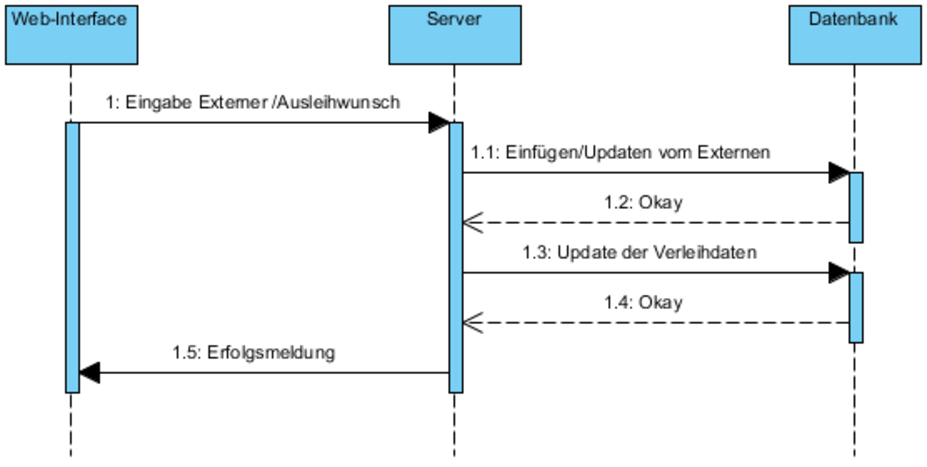
\includegraphics[width=0.8\linewidth]{bilder/Seq-Ausleihe.pdf}
\caption{Sequenzdiagramm für Ausleihe an Externe}
\label{fig:221}
\end{center}
\end{figure}


\section{Analyse von Funktion F222: Ausleihe übertragen}
\label{f:222}
Ein Dokument wechselt den Ausleihenden. Dabei muss ein Benutzer $A$ ein von ihm ausgeliehenes Dokument auswählen und einem anderen Benutzer $B$ übertragen. Alternative kann Benutzer $B$ auch eintragen, dass er sich ein Dokument von Benutzer $A$ geholt hat, das Dokument also jetzt bei ihm zu finden ist. Das System vermerkt dieses Austausch dann in der Datenbank mittels einer Built-In-Funktion von Django. Auch diese Funktion gehört zur \textbf{View}-Komponente mit Zugriff auf die \textbf{DB}.

Auch dieses Sequenzdiagramm gleicht sehr der Abb.\ \ref{fig:221}. Bei dieser Funktion muss vorher allerdings darauf geprüft werden, ob das Dokument wirklich ausgeliehen ist (auch nur eine Suchanfrage). Außerdem entfallen wieder 1.1 und 1.2.

\section{Analyse von Funktion F223: Ausleihe zurückgeben}
\label{f:223}
Ein Benutzer braucht ein Dokument nicht mehr und gibt es in den Bestand der Bibliothek zurück. Auch hierfür muss der Benutzer als Entleiher des Dokumentes eingetragen sein. Wenn dies der Fall sein sollte, kann er \emph{zurückgeben} wählen und das Dokument wird auch im Datensatz mittels Built-In-Funktionen von Django mit dem Status 0 versehen. Die Funktion ist dem \textbf{View} zugeordnet, benötigt aber auch die \textbf{DB}.

Wieder auf Abb. \ref{fig:221} berufend, muss hier vorher geprüft werden, ob der Benutzer auch wirklich das Dokument ausgeliehen hat, 1 muss "Rückgabewunsch" und 1.1 und 1.2 wird wieder weggelassen.

\section{Analyse von Funktion F224: (Optional) Ausleihe vermisst melden}
\label{f:224}
Das Dokument befindet sich nicht mehr an dem laut Datenbank befindlichen Ort. Dann kann ein Benutzer ein Dokument auf der Dokumentenansicht als \emph{vermisst} melden und dieses wird in der Datenbank mittels Statusänderung vermerkt. Dazu wird eine E-Mail an alle Benutzer verschickt oder alternativ eine Meldung auf der Homepage angezeigt. Hierfür muss eine neue App erstellt werden, die den Status ändert, die E-Mail-Adressen, den -Text und die Dokumentinformationen aufruft, verarbeitet und an alle verschickt oder alternativ einen entsprechenden Beitrag auf der Homepage erstellt. Das Ganze gehört dann zu \textbf{View} und \textbf{DB}.

Das dazugehörige Sequenzdiagramm ist Abb.\ \ref{fig:224}.
\begin{figure}
\begin{center}
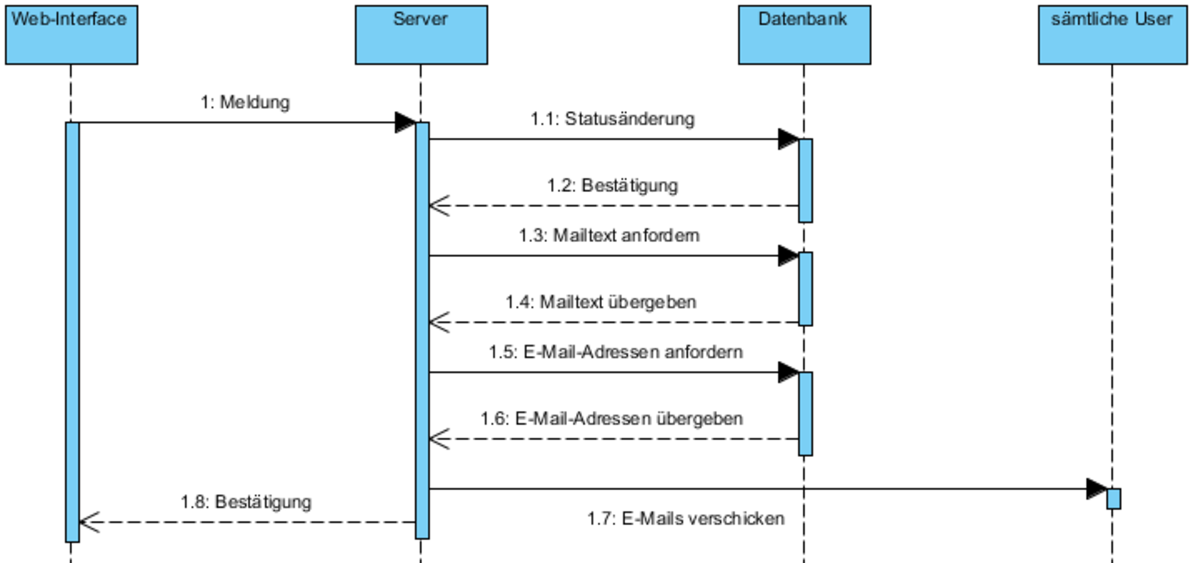
\includegraphics[width=0.8\linewidth]{bilder/Seq-Vermisst.pdf}
\caption{Sequenzdiagramm für eine Vermisstmeldung}
\label{fig:224}
\end{center}
\end{figure}

\section{Analyse von Funktion F225: Ausleihe verloren melden}
\label{f:225}
Das Dokument ist auch nach einer Vermisstenmeldung nicht wieder aufgetaucht. Dann ist ein Bibliothekar berechtigt, es als \emph{verloren gegangen} einzustufen. Das Dokument bekommt den entsprechenden Status und wird demnächst bei weiteren Suchanfragen ausgeschlossen. Dies erfolgt wieder innerhalb der \textbf{View}- und \textbf{DB}-Komponenten durch eine Built-In-Funktion von Django.

<<<<<<< HEAD
Das gewünschte Sequenzdiagramm ist ähnlich dem von Abb.\ \ref{fig:224}. Dabei muss nur vorher geprüft werden, ob der Nutzer die entsprechenden Rechte besitzt, und 1.3 bis 1.7 entfällt.
=======
Bei dieser Funktion ist das Sequenzdiagramm auch trivial. Es wird wieder erst gesucht (Abb. \ref{fig:Seqü)}, geprüft, ob das Dokument vermisst wird und der Benutzer ausreichende Rechte besitzt, und schließlich der Status der Literatur geändert. 
>>>>>>> 3f2da0a052b2b4c2920f7378594f577a485deecb
